\subsubsection{Fase complessiva}

\subsubsubsection{Prospetto orario}
Distribuzione delle ore per ciascun ruolo nel periodo di Progettazione di dettaglio e codifica:

\rowcolors{2}{lightRowColor}{darkRowColor}
\begin{longtable}{
		>{\centering}p{0.25\textwidth}
		>{\centering}p{0.05\textwidth}
		>{\centering}p{0.05\textwidth}
		>{\centering}p{0.05\textwidth}
		>{\centering}p{0.05\textwidth}
		>{\centering}p{0.05\textwidth}
		>{\centering}p{0.05\textwidth}
		>{\centering\arraybackslash}p{0.15\textwidth} }
	
	\coloredTableHead
	\textbf{\color{white}Nome} &
	\textbf{\color{white}Rp} &
	\textbf{\color{white}As} &
	\textbf{\color{white}An} &
	\textbf{\color{white}Pt} &
	\textbf{\color{white}Pr} &
	\textbf{\color{white}Vf} &
	\textbf{\color{white}Totale}
	\tabularnewline
	\endhead
	
	% Contenuto della tabella
	% Nome & Rp & As & An & Pt & Pr & Vf & Totale \\
	\VB & 7 & 4 & - & 6  & 20 & 12 & 49 \\
	\LB & - & - & - & 15 & 20 & 14 & 49 \\
	\NF & - & 8 & - & 12 & 19 & 10 & 49 \\
	\EG & 6 & - & - & 15 & 20 & 8  & 49 \\
	\FJ & 5 & 5 & - & 10 & 19 & 10 & 49 \\
	\MP & 5 & 6 & - & 8  & 15 & 15 & 49 \\
	\AS & - & - & - & 14 & 20 & 15 & 49 \\
	\AZ & - & 9 & - & 8  & 20 & 12 & 49 \\
	\textbf{Ore totali per ruolo} & 23 & 32 & - & 88 & 153 & 96 & 392 \\
	
	\rowcolor{white}\caption {Suddivisione oraria del periodo di Progettazione di dettaglio e codifica} \\
	
\end{longtable}

% Grafico
Rappresentazione grafica della suddivisione oraria:
\begin{figure}[H]
	\centering
	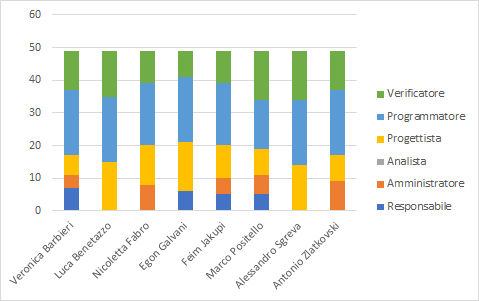
\includegraphics[width=0.7\textwidth]{./res/img/progettazioneDettaglioCodifica_po.png}
	\caption{Suddivisione oraria del periodo di Progettazione di dettaglio e codifica}
\end{figure}


\subsubsubsection{Prospetto economico}
	Totale delle ore e costo per ciascun ruolo nel periodo di Progettazione di dettaglio e codifica:

	\rowcolors{2}{lightRowColor}{darkRowColor}
	\begin{longtable}{
		>{\centering}p{0.25\textwidth}
		>{\centering}p{0.05\textwidth}
		>{\centering\arraybackslash}p{0.15\textwidth} }

		\coloredTableHead
		\textbf{\color{white}Ruolo} &
		\textbf{\color{white}Ore} &
		\textbf{\color{white}Costo in \euro{}}
		\tabularnewline
		\endhead

		% Contenuto della tabella
		% Ruolo & Ore & Costo \\
		Responsabile    & 23 & 690,00 \\
		Amministratore  & 32 & 640,00 \\
		Analista        & -  & - \\
		Progettista     & 88 & 1.936,00 \\
		Programmatore   & 153 & 2.295,00 \\
		Verificatore    & 96  & 1.440,00 \\
		\textbf{Totale} & 392 & 7.001,00 \\

		\rowcolor{white}\caption {Prospetto dei costi per il periodo di Progettazione di dettaglio e codifica} \\

	\end{longtable}

	% Grafico
	Rappresentazione grafica della distribuzione dei ruoli:
	\begin{figure}[H]
		\centering
		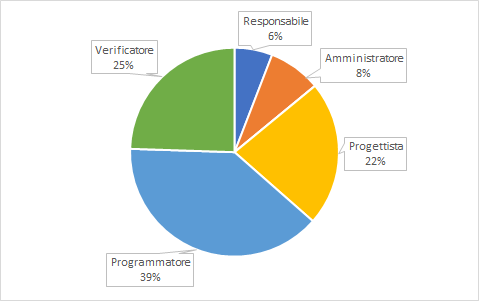
\includegraphics[width=0.7\textwidth]{./res/img/progettazioneDettaglioCodifica_pe.png}
		\caption{Suddivisione dei ruoli nel periodo di Progettazione di dettaglio e codifica}
	\end{figure}